\documentclass[11pt]{article}
\usepackage[margin=1in]{geometry}
\usepackage{graphicx}

\title{Checkpoint 1: Bitcoin-Led Cross-Asset Signals}
\author{HEX Research | Ethan Tait and Hank Rugg}
\date{November 9, 2026}

\begin{document}
\maketitle

\section*{Objective} Test whether a simple forecast of a follower's next-minute BTC-hedged return can improve execution relative to beta-hedged TWAP. The universe is BTC, ETH, SOL, XRP, and DOGE Binance perpetual futures. The descriptive survey uses 2023; monthly walk-forward comparisons use 2024. The 2025 holdout remains reserved. Stale prices are masked before calculating returns, including the return immediately after a stale bar.

\section{Price features and EMA horizons}
The price feature is an exponentially weighted mean of one-minute mid-price log returns, in basis points, with half-lives of 1, 3, and 5 minutes. Correlation matrices use common valid minutes in 2023.
\begin{figure}[htbp]
\centering
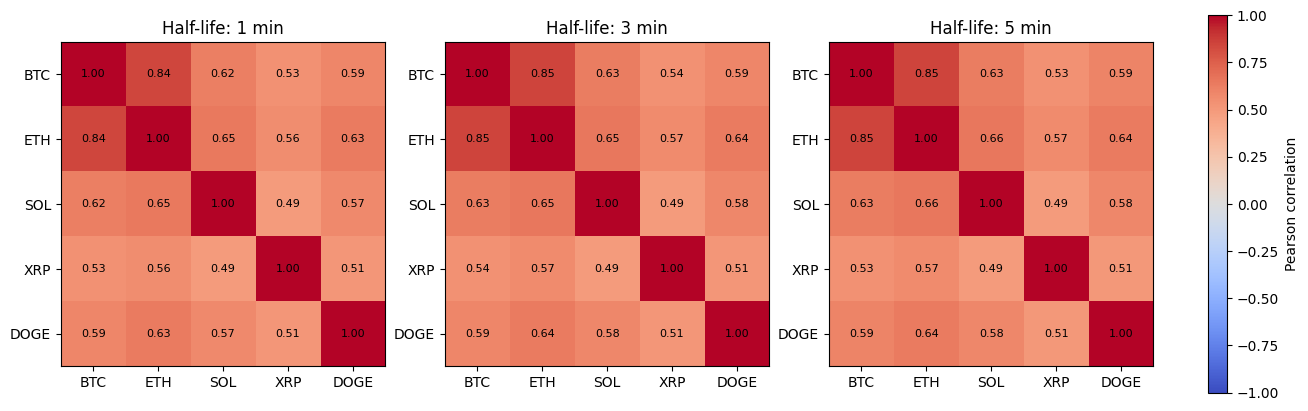
\includegraphics[width=\textwidth]{images/ema-correlations.png}
\caption{Contemporaneous return-EMA correlations at three half-lives.}\label{fig:ema}
\end{figure}

The correlation structure changes little across these horizons: BTC--ETH stays near 0.84--0.85, while BTC's correlations with the other followers range from about 0.53 to 0.63. The 3-minute half-life is preselected as a middle ground. These correlations describe common movement; they do not establish predictive lead--lag.

\section{Typical versus high-volatility conditions}
For the chosen half-life, daily correlation matrices are averaged with equal weight per day. Eligible days have at least 95\% common return coverage. The high-volatility day maximizes BTC realized volatility, measured by the square root of summed squared minute returns.
\begin{figure}[htbp]
\centering
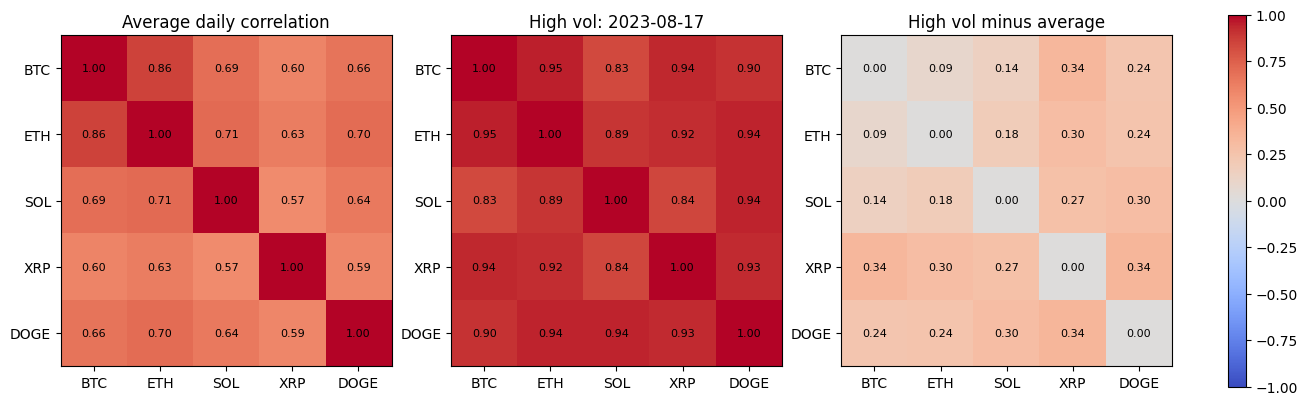
\includegraphics[width=\textwidth]{images/high-volatility.png}
\caption{Average daily correlation, August 17, 2023, and their difference.}\label{fig:vol}
\end{figure}

On August 17, correlations rise across all pairs. BTC--XRP increases from about 0.60 on the average day to 0.94; BTC--DOGE rises from 0.66 to 0.90. Common market exposure is therefore especially prominent on this selected stress day. One day illustrates this contrast; it does not establish a general regime effect.

\section{Volume-weighted index}
Each day's weights use the prior day's approximate USDT turnover (base volume times minute mid-price). The index return is the weighted sum of simple returns. Histograms use common valid 2023 minutes; the displayed range omits extreme tails.
\begin{figure}[htbp]
\centering
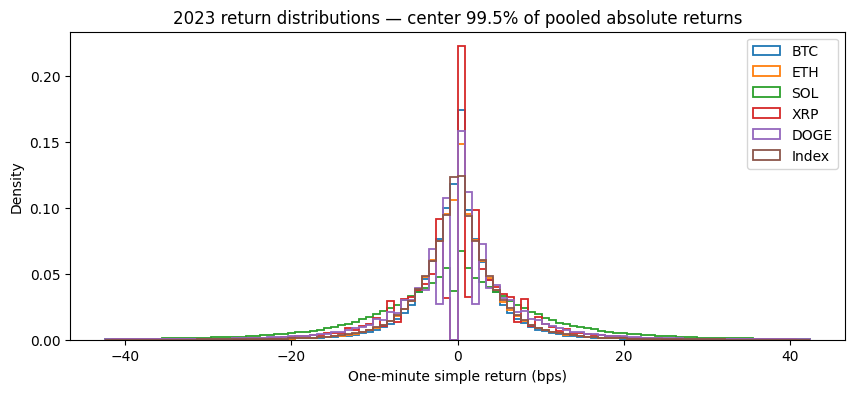
\includegraphics[width=0.80\textwidth]{images/return-distributions.png}
\caption{One-minute return distributions for five instruments and the volume-weighted index.}\label{fig:hist}
\end{figure}

Returns are sharply peaked and heavy-tailed. Full-sample minute-return standard deviations are about 6.2 bps for BTC, 14.2 bps for SOL, and 6.6 bps for the index. The index is less volatile than the smaller coins, but not less volatile than BTC.

\section{Forecast and improvement loop}

\subsection{What we predict}
For each follower (ETH, SOL, XRP, and DOGE), the model predicts its next-minute move after removing its estimated BTC exposure:
\[
y_{i,t+1}=r_{i,t+1}-\beta_{i,t}r_{\mathrm{BTC},t+1}.
\]
Returns are one-minute mid-price log returns in bps. Beta is follower--BTC covariance divided by BTC variance, using 60 valid paired minutes through $t-1$. This known beta defines the next-minute target; no intercept is subtracted. If beta is 1.5, BTC rises 2 bps, and the follower rises 4 bps, the target is $4-1.5(2)=1$ bp: the follower outperformed its BTC exposure.

\subsection{The three models}
All three are linear ridge regressions, fitted separately for each follower. Ridge fits an intercept and feature coefficients while penalizing large coefficients; its fixed penalty is 10. Predictors are standardized using the training period's means and standard deviations.
\begin{enumerate}
\item \textbf{BTC EMA only.} Use the 3-minute-half-life EMA of BTC's one-minute returns. This tests whether BTC's recent direction predicts the follower's next BTC-adjusted move.
\item \textbf{Add own EMA.} Keep BTC EMA and add the same return EMA for the follower. This controls for the follower's own recent movement and allows momentum or reversal to contribute.
\item \textbf{Add flow.} Keep both return EMAs and add a 3-minute-half-life EMA of the follower's trade imbalance, $(V_{\mathrm{buy}}-V_{\mathrm{sell}})/(V_{\mathrm{buy}}+V_{\mathrm{sell}})$. This tests whether buying or selling pressure adds information beyond prices.
\end{enumerate}

\subsection{How forecasts change execution}
For each follower and eligible day, generate one buy and one sell at random valid start minutes using seed 42. Every parent order has \$10,000 arrival notional and 30 one-minute execution opportunities. All models and beta-hedged TWAP face the same orders. Only complete windows with valid prices and forecasts are used.

The parent order is assumed to exist already: the forecast decides how quickly to fill it, not whether to buy or sell. At each minute, divide the remaining coin quantity by the number of execution opportunities left to obtain the neutral child quantity. TWAP uses this quantity without a signal adjustment.

For example, suppose the parent order is to buy \$10,000 of SOL over 30 minutes. Initially, the neutral child is one-thirtieth of the total SOL quantity, worth approximately \$333 at the arrival price. A predicted BTC-hedged return of $+0.25$ bps gives a multiplier of $1+0.25=1.25$, so the first child buys approximately \$417 worth. A forecast of $-0.25$ bps gives a multiplier of $0.75$, or approximately \$250 worth. The actual calculation uses coin quantities; these dollar amounts illustrate the first decision at the arrival price.

The multiplier is bounded between 0.5 and 1.5. For a sell, reverse the forecast's sign: a positive forecast encourages waiting, while a negative forecast accelerates selling. Recalculate the neutral quantity and forecast adjustment every minute from what remains. No child exceeds the remaining quantity, and the final child fills everything left to guarantee completion. These are simulated fills at the next minute's ask for buys or bid for sells.

Both schedules open a BTC hedge at arrival, with signed notional equal to side times arrival beta times target arrival notional. For positive beta, this means long BTC while waiting to buy and short BTC while waiting to sell. Beta is frozen for the order, and each target fill closes the corresponding fraction of the hedge. Bid/ask fills and 5 bps transaction fees apply to both legs. Market impact and funding are omitted.

\subsection{How we compare the iterations}
For each order, net hedged implementation shortfall is the side-adjusted target fill cost relative to arrival mid-price, plus target fees, minus net BTC hedge P\&L normalized by target arrival notional. Hedge P\&L includes its trading costs. Improvement equals TWAP's net shortfall minus the signal schedule's net shortfall, so positive values favor the signal.

Average order improvements within each UTC day, then compare the median daily improvement across versions. Resample whole days 1,000 times to obtain descriptive 95\% bootstrap intervals. The left plot shows these medians and intervals; the right sums daily average improvements over time. It is an execution comparison, not compounded portfolio P\&L.

\begin{figure}[htbp]
\centering
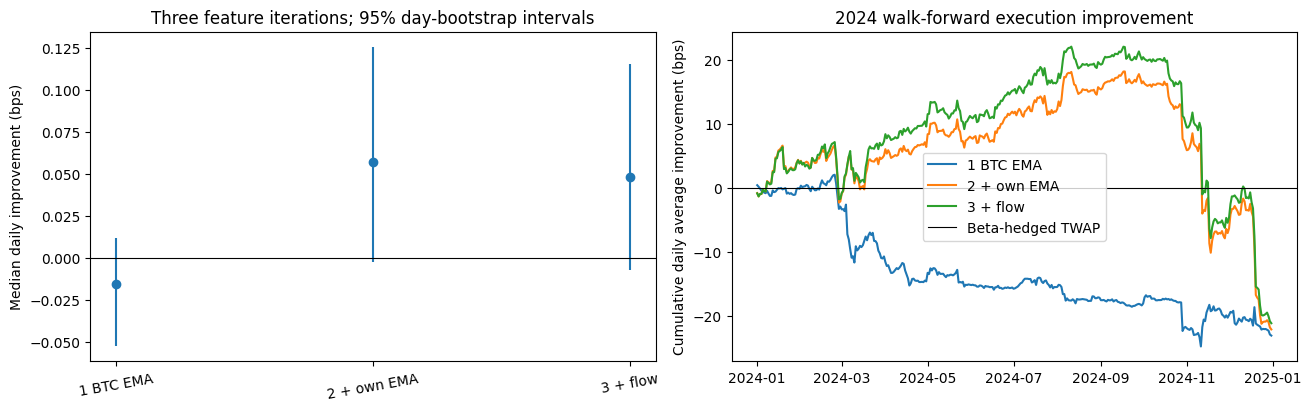
\includegraphics[width=\textwidth]{images/execution-results.png}
\caption{Median daily net improvement with 95\% day-bootstrap intervals (left); cumulative daily average improvement versus beta-hedged TWAP (right). The cumulative series is not portfolio P\&L.}\label{fig:execution}
\end{figure}

\section*{Findings} Median daily improvement is $-0.0153$, $0.0574$, and $0.0481$ bps for versions 1--3. Own-return information improves forecast ranking; flow adds little consistently. All 95\% intervals include zero, and larger losses leave every cumulative curve below TWAP. This MVP does not demonstrate an execution advantage. Next, inspect late-year losses and test an own-return-only baseline. Results depend on synthetic-order assumptions; the bootstrap treats days as independent.

\end{document}
